\textbf{Only if we assume the classification scheme as shown in Figure \ref{fig:problem_2}:}

\begin{figure*}[!ht]
	\centering
	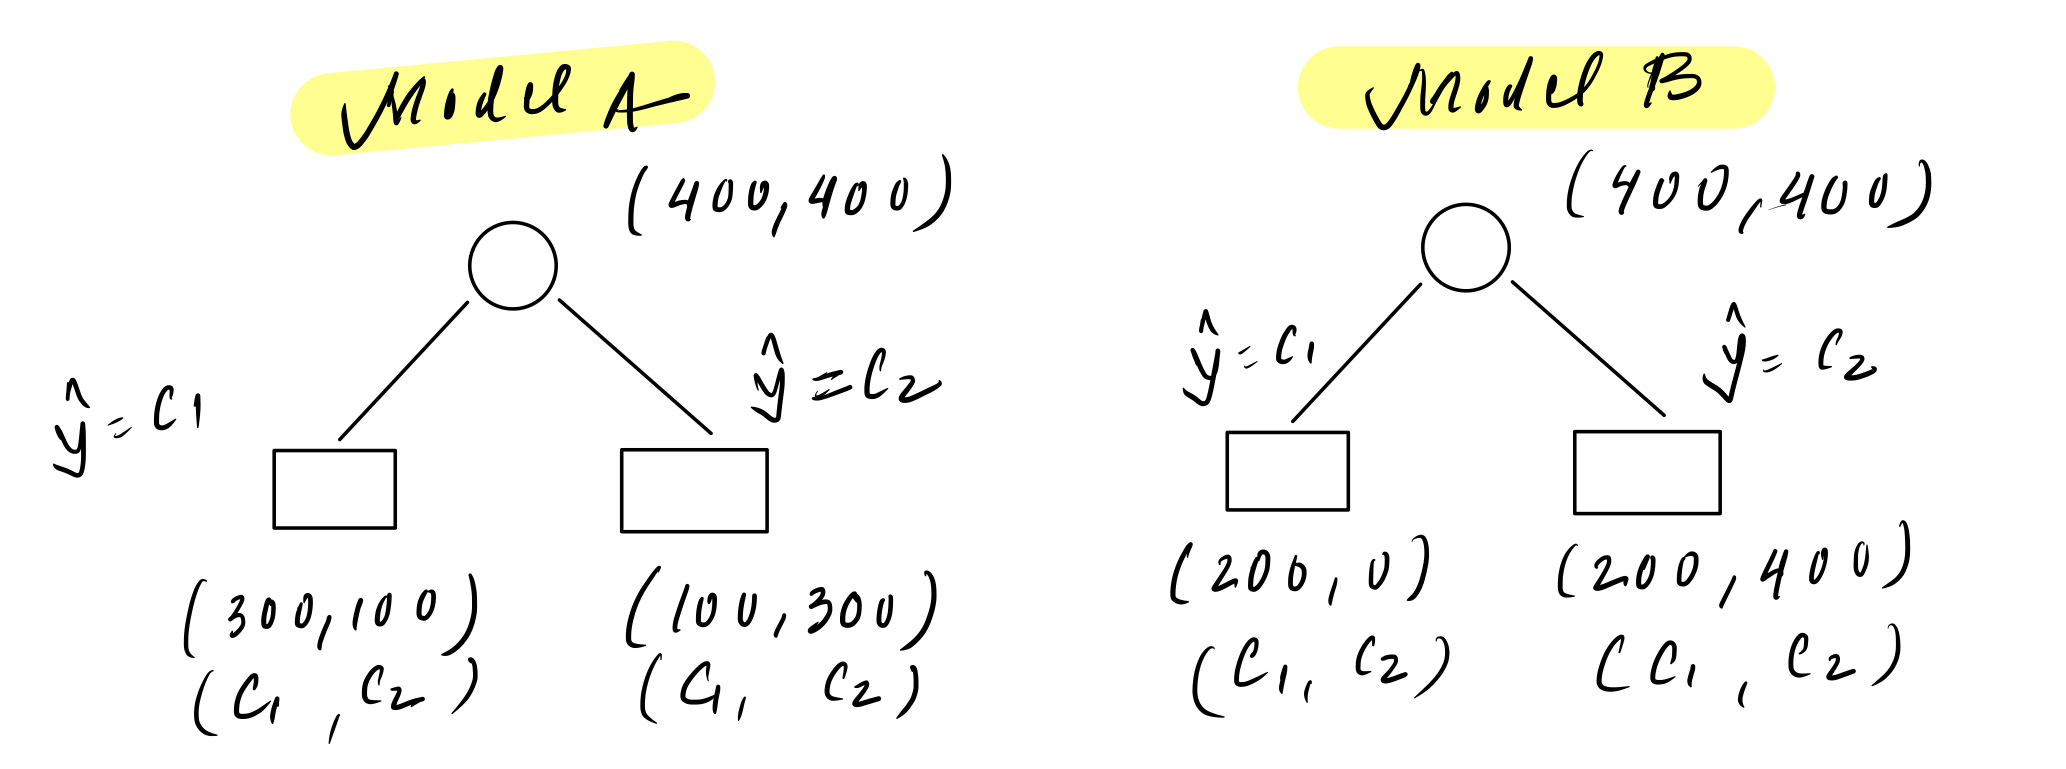
\includegraphics[width=0.75\textwidth]{images/problem_2.jpeg}
	\caption{Decision tree classification scheme}
	\label{fig:problem_2}	
\end{figure*}

\begin{align*}
	\delta_{Model A} & = \frac{100 + 100}{400 + 400} = 0.25 \\
	\delta_{Model B} & = \frac{0 + 200}{400 + 400} = 0.25 \\
\end{align*}

We can show that the misclassification rates are equal.
	
\textbf{Cross-entropy:}

Let $y_{C_{1}} = 0$ and $y_{C_{2}} = 1$

For Model A
\begin{align*}
	\mathcal{CE} & = - [ \sum_{i=1}^{n} y_{i} \log p + (1 - y_{i}) \log (1 - p) ] \\
	\mathcal{CE}_{C_{1}} & = - [ 0 \log (0.75) + (1 - 0) \log (1 - 0.75) ] = 1.39 \\
	\mathcal{CE}_{C_{2}} & = - [ 1 \log (0.25) + (1 - 1) \log (1 - 0.25) ] = 1.39 \\	
	\mathcal{CE} & = 1.39 + 1.39 = 2.78
\end{align*}


For Model B
\begin{align*}
	\mathcal{CE}_{C_{1}} & = - [ 0 \log (1) + (1 - 0) \log (1 - 1) ] = 0 \\
	\mathcal{CE}_{C_{2}} & = - [ 1 \log (0.33) + (1 - 1) \log (1 - 0.33) ] = 1.11 \\	
	\mathcal{CE} & = 0 + 1.11 = 1.11
\end{align*}

\textbf{Gini Index:}

For Model A
\begin{align*}
	\text{Gini}(\text{Model A}) = 1 - \left[ \left( \frac{400}{800} \right)^{2} + \left( \frac{400}{800} \right)^{2}  \right] = 0.5
\end{align*}

For Model B
\begin{align*}
	\text{Gini}(\text{Model B}) = 1 - \left[ \left( \frac{200}{800} \right)^{2} + \left( \frac{600}{800} \right)^{2} \right] = 0.375
\end{align*}

Both cross-entropy and gini index are lower for Model B,
